% Schematic of the two nested minimizations of Appendix C: the outer BFGS loop over the
% frame S (C.3) wraps the inner self-consistent product-state loop (C.2); the converged
% self-consistent product state exits as the C-normalized optimum S*. Loop labels carry \cref
% references to main.tex equations, so a standalone compile shows them as ??. \input into main.tex via the standalone package.
\documentclass[border=3pt]{standalone}
\usepackage{amsmath,amssymb,braket}
\usepackage{hyperref}
\usepackage[noabbrev]{cleveref}
\usepackage{tikz}
\usetikzlibrary{arrows.meta,positioning,fit,calc}
\newcommand{\costFunc}{\mathcal{F}}
\begin{document}
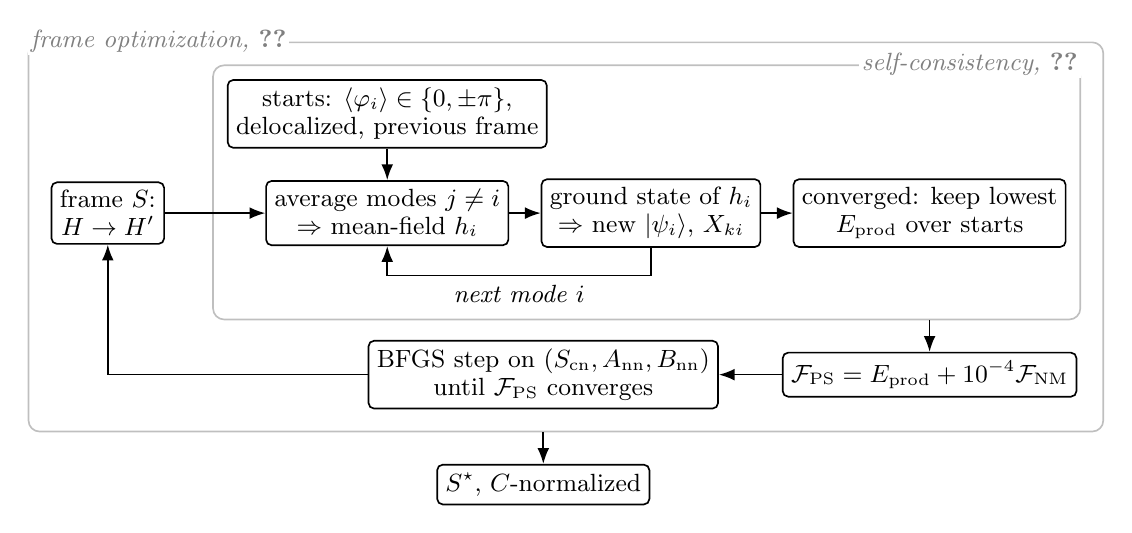
\begin{tikzpicture}[
    font=\small,
    box/.style={draw, rounded corners=2pt, align=center, inner sep=3pt, line width=0.6pt, fill=white},
    loop/.style={draw=gray, draw opacity=0.5, rounded corners=4pt, inner sep=5pt, line width=0.6pt},
    looplab/.style={font=\small\itshape, inner sep=1pt, fill=white, text=gray, text opacity=1, draw opacity=1},
    arr/.style={-{Latex[length=2mm]}, line width=0.6pt},
    lab/.style={font=\small\itshape, inner sep=1pt, fill=white},
    node distance=4mm and 4mm,
]
    % ---- inner loop: starts feed a horizontal ring, converged solutions leave to the right ----
    \node[box] (hi) {average modes $j\neq i$\\[-1pt] $\Rightarrow$ mean-field $h_i$};
    \node[box, right=of hi] (psi) {ground state of $h_i$\\[-1pt] $\Rightarrow$ new $\ket{\psi_i}$, $X_{ki}$};
    \node[box, right=of psi] (keep) {converged: keep lowest\\[-1pt] $E_{\rm prod}$ over starts};
    \node[box, above=of hi] (starts) {starts: $\langle\varphi_i\rangle\in\{0,\pm\pi\}$,\\[-1pt] delocalized, previous frame};
    \draw[arr] (starts) -- (hi);
    \draw[arr] (hi) -- (psi);
    \draw[arr] (psi) -- (keep);
    \coordinate (ret) at ($(psi.south)+(0,-3.5mm)$);
    \draw[arr] (psi.south) -- (ret) -| (hi.south);
    \node[lab, below=0.8mm of {$(ret)!0.5!(ret -| hi.south)$}] (retlab) {next mode $i$};
    \node[loop, fit=(starts)(hi)(psi)(keep)(retlab), label={[looplab, anchor=east]north east:self-consistency, \cref{eq:mean_field_h}}] (inner) {};
    % ---- outer loop: frame on the left, cost and BFGS snaking back below ----
    \node[box, left=6mm of hi.west -| inner.west] (frame) {frame $S$:\\[-1pt] $H\to H'$};
    \draw[arr] (frame) -- (hi);
    \node[box, anchor=north] (cost) at ($(inner.south -| keep.center)+(0,-4mm)$) {$\costFunc_{\rm PS}=E_{\rm prod}+10^{-4}\costFunc_{\rm NM}$};
    \draw[arr] (inner.south -| keep.center) -- (cost);
    \node[box, left=8mm of cost] (bfgs) {BFGS step on $(S_{\rm cn},A_{\rm nn},B_{\rm nn})$\\[-1pt] until $\costFunc_{\rm PS}$ converges};
    \draw[arr] (cost) -- (bfgs);
    \draw[arr] (bfgs.west) -| (frame.south);
    \node[loop, inner sep=8pt, fit=(frame)(inner)(cost)(bfgs), label={[looplab, anchor=west]north west:frame optimization, \cref{eq:H_frame}}] (outer) {};
    % ---- exits ----
    \node[box, anchor=north] (sopt) at ($(outer.south -| bfgs.center)+(0,-4mm)$) {$S^\star$, $C$-normalized};
    \draw[arr] (outer.south -| bfgs.center) -- (sopt);
\end{tikzpicture}
\end{document}
